\documentclass{article}
\usepackage[english]{babel}
\usepackage{etoolbox}
\usepackage{pgfplots}
\usetikzlibrary{arrows}
\usepackage[utf8]{inputenc}
\usepackage[margin=0.5in]{geometry}
\usepackage{bbold}
\usepackage{amsmath}
\usepackage{graphicx}
\usepackage{amsmath}
\usepackage[makeroom]{cancel}
\graphicspath{ {./images/} }
\renewcommand{\arraystretch}{3}
\usepackage{xcolor}
\setlength\parindent{0pt}
\newcommand*{\Perm}[2]{{}^{#1}\!P_{#2}}%
\newcommand*{\Comb}[2]{{}^{#1}C_{#2}}%

\title{Probability Question - Playoff Series}
\author{David Veitch}
\date{September 2018}

\begin{document}

\maketitle

\section{Question}

Team A faces Team B in a best of seven playoff series. For each game, assume Team A has probability $a$ of winning ($a \in \mathbb{R}, 0 \leq a \leq 1$). What is the probability that Team A wins the series?

\section{Answer}

For Team A to win, it must win four games. There are four ways this can happen; that is, Team A can win the series in four, five, six, or seven games.\\

Obviously the probability Team A wins in four games is:

\begin{equation} 
\begin{split}
P(\text{A Wins In 4}) &= (a)(a)(a)(a) = (a)^{4}\\
\end{split}
\end{equation}

Team A winning in more than four games is slightly more complicated. Note that if team A wins in five games, this means Team A wins three out of the first four games, and then wins the fifth and final game. There are $\binom 43=\frac{4!}{3!1!} = 4$ ways for Team A to win three out of the first four. Therefore:

\begin{equation} 
\begin{split}
P(\text{A Wins In 5}) &= \left[ \binom 43(a)(a)(a)(1-a) \right](a)  = \binom 43 (a)^{4} (1-a)\\
\end{split}
\end{equation}

Similarly we have:

\begin{equation} 
\begin{split}
P(\text{A Wins In 6}) &=  \binom 53 (a)^{4} (1-a)^2\\
\end{split}
\end{equation}
\begin{equation} 
\begin{split}
P(\text{A Wins In 7}) &=  \binom 63 (a)^{4} (1-a)^3\\
\end{split}
\end{equation}

We are interested in the probability Team A wins the series. Since Team A winning in four, five, six, or seven games are disjoint events, we can use finite additivity (the probability of any of these events occuring is equal to the summation of the individual probabilities):

\begin{equation} 
\begin{split}
P(\text{A Wins The Series}) &=  P(\text{A Wins In 4}) + P(\text{A Wins In 5}) + P(\text{A Wins In 6}) + P(\text{A Wins In 7})\\
\end{split}
\end{equation}

\newpage

\section{Supplemental Material}

I like this question for two reasons.\\

First, it is a fairly straightforward probability question, but with one interesting trick (that is one must realize that if Team A wins the series it is guaranteed that Team A wins the final game).\\

Second, it has real world implications. Who doesn't get excited when playoff hockey/basketball/baseball series are being played! What I find interesting is that even small differences in per-game probabilities can lead to big differences in the probability one team or the other wins the series. For example if Team A has a 60\% chance of winning each individual game, the probability of Team A winning the series is 71\%.\\

\begin{center}
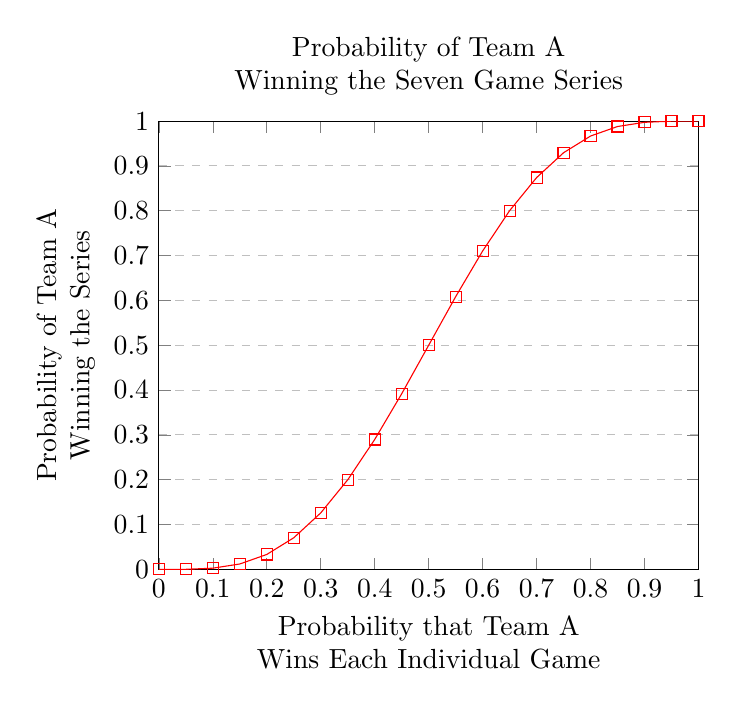
\begin{tikzpicture}
\begin{axis}[
    title={Probability of Team A\\ Winning the Seven Game Series},
    title style={align=center},
    xlabel={Probability that Team A\\ Wins Each Individual Game},
    xlabel style={align=center},
    ylabel={Probability of Team A\\ Winning the Series},
    ylabel style={align=center},
    xmin=0, xmax=1,
    ymin=0, ymax=1,
    xtick={0,.1,.2,.3,.4,.5,.6,.7,.8,.9,1},
    ytick={0,.1,.2,.3,.4,.5,.6,.7,.8,.9,1},
    legend pos=north west,
    ymajorgrids=true,
    grid style=dashed,
]
 
\addplot[
    color=red,
    mark=square,
    ]
    coordinates {
    (0,0)
    (0.05,0.000193578)
    (0.1,0.002728)
    (0.15,0.012103172)
    (0.2,0.033344)
    (0.25,0.070557)
    (0.3,0.126036)
    (0.35,0.199845734)
    (0.4,0.289792)
    (0.45,0.391712203)
    (0.5,0.5)
    (0.55,0.608287797)
    (0.6,0.710208)
    (0.65,0.800154266)
    (0.7,0.873964)
    (0.75,0.929443359)
    (0.8,0.966656)
    (0.85,0.987896828)
    (0.9,0.997272)
    (0.95,0.999806422)
    (1,1)

    };

\end{axis}
\end{tikzpicture}
\end{center}

\end{document}
